\chapter{Spark自动缓存模块设计与实现}\label{chap:auto-cache}

\section{Spark相关模块现状分析}
Spark框架相对于Hadoop的核心改进是添加了缓存管理模块。通过将计算过程中的中间数据缓存在内存中可以极大的加速计算过程。尤其对于机器学习和图计算等迭代式计算有上百倍的加速效果。这是因为这种迭代式计算需要多次重复访问中间数据,就非常能体现Spark框架的优势。

\subsection{缓存模块底层原理}
Spark应用在执行过程中会将应用程序解析成DAG图,然后根据DAG的拓扑排序顺序执行DAG图中的每一个操作。一个RDD数据被计算得到之后,会存放在Execution Memory区域。如果没有立即被使用使用到就会从Execution Memory区域被删除。Spark框架给应用程序员提供了cache接口,cache接口会将RDD对象的STORAGE\_LEVEL字段标记为MEMORY\_ONLY。标记之后Spark框架并不会立即缓存数据,而是在RDD分区数据计算完成时查看STORAGE\_LEVEL标记。根据不同的标记将数据缓存到不同的位置,常见的标记有以下几种,MEMORY\_ONLY,DISK\_ONLY,MEMORY\_AND\_DISK。如果标记为MEMORY\_ONLY框架就会将数据缓存到内存之中,具体过程是将RDD的应用发送给BlockManager对象的MemoryStore模块。MemoryStore模块会保存RDD模块的引用。这样就能将RDD对象长时间保存在内存中。从缓存管理模块的逻辑视图角度来看cache接口调用是将RDD对象从Execution Memory区域移到了Storage Memory区域。如果STORAGE\_LEVEL标记为DISK\_ONLY。框架会将RDD对象的引用发送给BlockManager的DiskStore模块。DiskStore模块在HDFS或者其他文件系统上创建一个文件,将RDD对象写入文件之中。并且保存文件的路径。这就是缓存管理模块的核心过程。

当要使用到一个RDD数据时,框架会从BlockManager模块查看数据是否存在缓存数据。此时有两种情况,如果缓存数据存放在磁盘之中框架会将数据读取加载到内存的Execution Memory区域。如果是缓存在内存之中就可以直接进行计算。

在分析了缓存模块的核心原理之后还有一个重要的问题,就是缓存决策是如何实现的。目前Spark应用的缓存决策全都由编程人员在开发的过程中手动指定。这存在着几个问题。第一,编程人员可能会做出不正确的缓存决定,缓存了无用的数据,这会导致内存被浪费,降低了系统内存资源的使用效率。第二,编程人员可能没有缓存重要数据,导致在计算的过程中重复计算重要数据,对应用程序的执行时间造成巨大的影响。第三,这种编程模式对Spark应用编程人员提出了比较高的要求,编程人员必须熟悉Spark框架的核心原理,还要熟悉Spark提供的众多算子的底层实现,在此基础上还需要在编程的过程中选择合适的数据进行缓存,在Spark应用程序规模变大之后就会对编程人员造成比较大的负担。

\subsection{自适应执行框架原理}
同时还需要考虑Spark框架最新的动态执行新特性。Spark框架本身是在不断发展之中,Spark这类并行数据处理系统存在着一些问题,下面三个问题对性能影响比较突出:

\begin{enumerate}
    \item shuffle partition 个数,比如spark的shuffle partition个数默认值为200。可以通过参数配置,这个参数决定了reduce阶段任务的数量,对整个查询的性能有很大的影响。假设一个查询运行前申请E个Executor,每个Executor包含C个core(并发执行线程数),那么该作业在运行时可以并行执行的作业个数就为$E\times C$个,也可以说该作业的并发数为$E\times C$个。假设shuffle partition个数为P,处理map stage的任务数和原始数据的文件数量和大小有关,后续的每个reduce stage的任务数量都为P。由于Spark作业调度是抢占式的,$E\times C$个作业会抢占执行P个任务,直至所有任务完成,就会进入下一个stage。在这个过程中,任务执行时间会过长,导致整个stage执行时间变长,另一方面,$E\times C$个执行单元大部分都处于空闲状态,导致整体资源利用率急剧下降。所以shuffle partition个数的设置就对性能有着很大的影响,在实际运行场景下,作业执行之前很难设置shuffle partion个数。
    \item 最佳执行计划,Spark SQL会将应用程序翻译成逻辑计划,然后经历一系列的优化,最后确定一个物理执行计划。最终选择的物理执行计划对性能有很大的影响。如果选择最佳的执行计划是Spark SQL的Catalyst优化器的核心工作。Catalyst早期主要是基于规则的优化器(RBO,Rule Based Optimizer),在Spark2.2中加入了基于代价的优化(CBO, Cost Based Optimizer)。也有一些工作实现了根据历史记录的优化(HBO,History Based Optimizer)。这些优化器统一的特点是在作业执行之前完全确定物理执行计划,一旦确定之后就不再改变。然而实际作业往往在事先无法完全预料。如图\ref{fig:wrong-sort-join}所示。其中一张表的大小仅为600KB,然后Spark申城的物理执行计划依旧使用了sortMergeJoin。这种场景明显使用BroadcastJoin更加合理。
    \item 数据倾斜问题。数据倾斜是常见的导致SparkSQL性能变差的问题。数据倾斜是指某一个partition的数据量远远大于其他partition的数据。导致个别任务的运行时间远远大于其他任务,因此拖累了整个作业的运行时间。在实际作业中,数据倾斜问题很常见,这是因为join key对应的hash值分布不均匀。在极端情况下,hash结果分布非常不均匀,导致大量数据被分到同一个partition二导致严重数据倾斜。如图\ref{fig:data-qinxie}所示,大部分任务在两秒内就完成了,但是最慢的任务却花了4分钟,这就是因为发生了数据倾斜问题,他处理的数据是其他任务的数倍。最终虽然大部分很快就运行结束,因为数据倾斜问题,整个作业的执行时间也被极大地影响了。

\end{enumerate}

\begin{figure}[htbp]
    \centering
    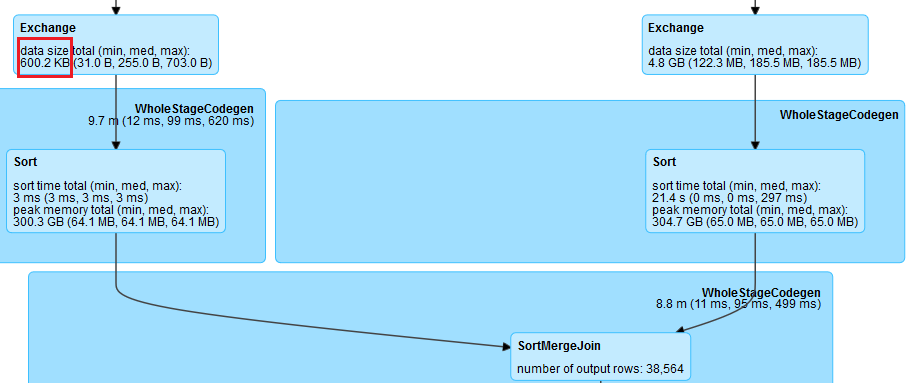
\includegraphics[width=0.99\textwidth]{Img/wrong-sort-join.png}
    \caption{不合理的物理执行计划}
    \label{fig:wrong-sort-join}
\end{figure}

\begin{figure}[htbp]
    \centering
    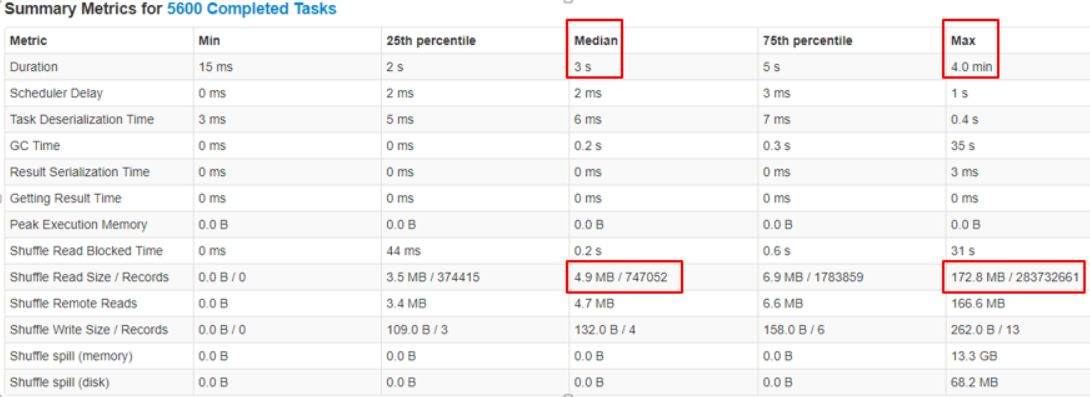
\includegraphics[width=0.99\textwidth]{Img/data-qingxie .png}
    \caption{数据倾斜问题}
    \label{fig:data-qinxie}
\end{figure}


对于这些问题,Spark设计实现了一套自适应执行框架。自适应执行框架的思路是在执行计划中划分好stage,然后按照stage提交执行,在运行过程中收集当前stage的统计信息,通过运行时信息来优化下一个stage的物理执行计划,然后提交后续的stage。在运行过程中,Spark动态执行框架会根据运行情况动态设置下游Reducer个数、动态调整执行计划、动态处理数据倾斜问题。

\section{自动缓存模块}

\subsection{自动缓存模块设计}
通过上文对Spark相关模块的详细分析后,本文设计了一种改进的自动缓存模块。需要实现自动缓存的功能,就需要能够判断在整个作业计算过程中哪些数据会被重复使用,对于需要重复使用的RDD数据,应该将其缓存在缓存之中,这样在之后的计算过程中,Spark框架就可以直接使用已经缓存的数据进行计算,从而能够加速计算过程。

针对Spark底层实现原理来分析,Spark会将应用程序转化为一个DAG图,这里使用$G(V, E)$来表示DAG。DAG图中的节点$V$是RDD数据,DAG图中的边$E$为RDD数据之间的转化关系,分为transformation和action两种。根据action操作,Spark框架会将整个DAG切分成多个作业,这里用$J={j_1, j_2,...,j_m }$表示所有作业。对于每个作业$j_i$,Spark框架会根据宽依赖将作业分为多个stage。如果$RDD_i$通过操作转化为$RDD_j$,其中存在一条边$(i, j)\in E$,那么$RDD_i$就称为$RDD_j$的父节点。对于$RDD_v$来说,它的所有父节点记为$anc(v)$。它的所有后继节点记为$dsc(v)$。

根据对Spark底层DAG图结构进行分析之后发现需要得到应用对应的DAG图,只要得到了DAG图,然后对DAG图进行分析就可以得到重复使用的RDD数据,在DAG图中,对于$RDD_v$, $dsc(v)$的大小就是会被重复使用的次数。在程序运行之前是很难得到DAG图结构,所以可以使用少量输入数据运行整个应用程序,然后记录DAG图结构。之后使用全量输入数据再次运行整个程序,这样就可以在第二次执行过程中缓存需要重复使用的数据。

在上文介绍了Spark的动态执行功能。动态执行功能会在执行过程中根据stage的运行时数据优化调整接下来的物理执行计划,所以当Spark调整执行计划时,自动缓存模块也需要同步更新修改DAG图结构,这样就可以保持正确的DAG图结构。

\subsection{自动缓存模块实现}
Spark应用程序都会创建一个SparkContext,SparkContext对应了一个Spark应用程序的生命周期,SparkContext中包含着RDD根节点,DAGScheduler,TaskScheduler,SchedulerBackend, BlockManager。本文所做的工作大多是修改SparkContext内的各个组件完成的。

SparkContext对象创建之后会初始化各个组件,初始化完成之后就会开始执行用户代码。Spark应用一般从读取数据开始,SparkContext提供了许多接口从文件系统中读取数据,Spark框架会创建一个新的RDD对象,在RDD对象的data字段存储这指向实际数据的应用。RDD对象有一个指向父节点的引用dependency, 输入节点RDD有一个特点,就是它的dependency是指向sparkContext对象的。所以sparkContext相当于是整个DAG图的根节点。

为了得到整个DAG图的结构,需要使用小量数据运行整个应用程序,得到DAG图结构。这就需要修改输入RDD节点,之前说过RDD节点是只读的,这种特性是利用了Scale语言的特性,将data字段设置为不可变的value对象。所以需要将data改为可变数据variable。这样就可以替换输入数据为小规模数据。同时还需要将全局RDD的STORAGE\_LEVEL字段设置为MEMORY\_ONLY,这是为了得到一个正确的DAG图结构。在计算结束之后,就可以得到完整的DAG图。Spark应用在结束的时候会调用sparkContext.stop接口结束整个应用并释放所有资源,所以可以修改stop接口,将数据替换为全量数据,重新运行整个作业之后结束整个作业。完整的流程如图\ref{fig:auto-cache}所示。

\begin{figure}[htbp]
    \centering
    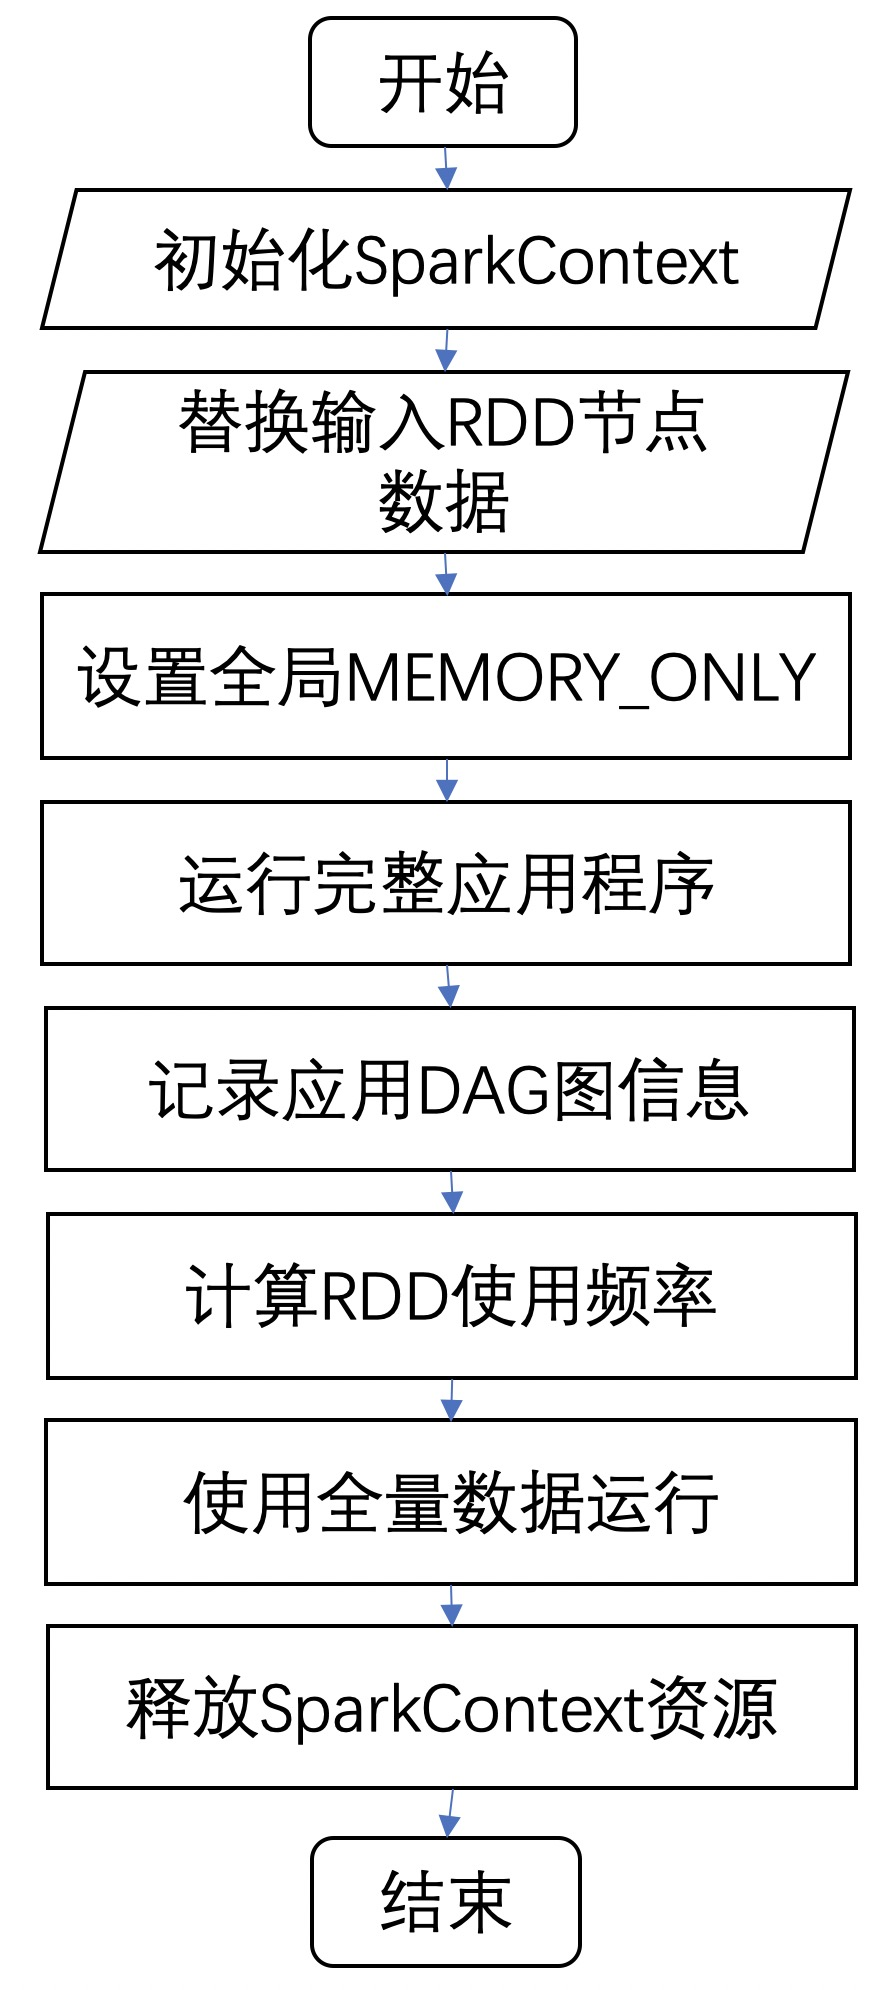
\includegraphics[width=0.4\textwidth]{Img/auto-cache.jpg}
    \caption{自动缓存流程图}
    \label{fig:auto-cache}
\end{figure}

RDD使用频率的算法如\ref{alg:mergesort}所示

\begin{algorithm}  
    \caption{用归并排序求逆序数}  
    \begin{algorithmic}[1] %每行显示行号  
        \Require $Array$数组,$n$数组大小  
        \Ensure 逆序数  
        \Function{Merger}{$Array, left, middle, right$}  
            \State $i\gets left$  
            \State $j\gets middle$  
            \State $k\gets 0$  
            \State $result \gets 0$  
            \While{$i<middle$ \textbf{and} $j<right$}  
                \If{$Array[i]<Array[j]$}  
                    \State $B[k++]\gets Array[i++]$  
                \Else  
                    \State $B[k++] \gets Array[j++]$  
                    \State $result \gets result + (middle - i)$  
                \EndIf  
            \EndWhile  
            \While{$i<middle$}  
                \State $B[k++] \gets Array[i++]$  
            \EndWhile  
            \While{$j<right$}  
                \State $B[k++] \gets Array[j++]$  
            \EndWhile  
            \For{$i = 0 \to k-1$}  
                \State $Array[left + i] \gets B[i]$  
            \EndFor  
            \State \Return{$result$}  
        \EndFunction  
    \end{algorithmic}
    \label{fig:mergesort}
\end{algorithm}
\section{自动缓存管理模块测试与性能分析}
\section{本章总结}


